%文中的Grid-LSTM模型做的语义图像分割的例子
\begin{figure}
	\centering
	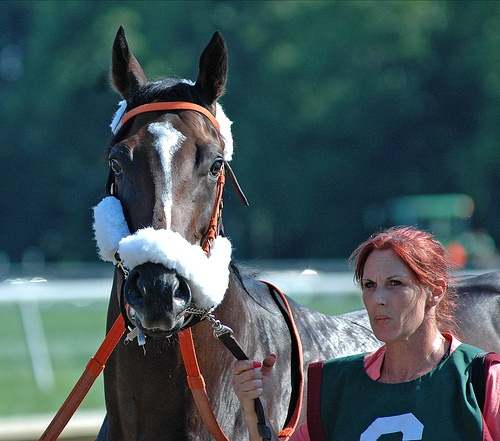
\includegraphics[width=.2\textwidth,height=.15\textwidth]{demo_images/example/2007_000799.jpg}
	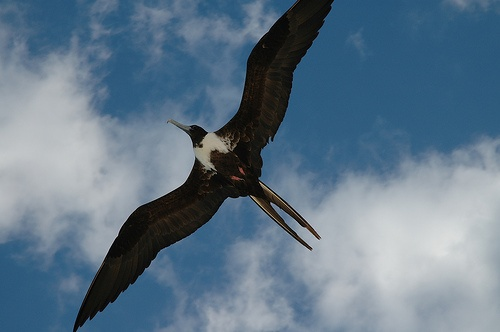
\includegraphics[width=.2\textwidth,height=.15\textwidth]{demo_images/example/2007_002094.jpg}
	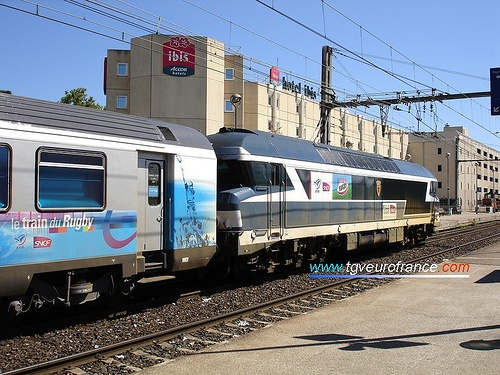
\includegraphics[width=.2\textwidth,height=.15\textwidth]{demo_images/example/2007_004483.jpg}
	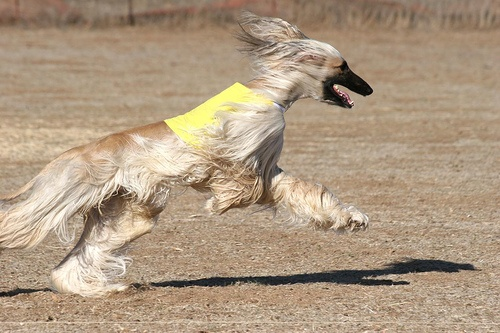
\includegraphics[width=.2\textwidth,height=.15\textwidth]{demo_images/example/2007_003194.jpg}
	\\
	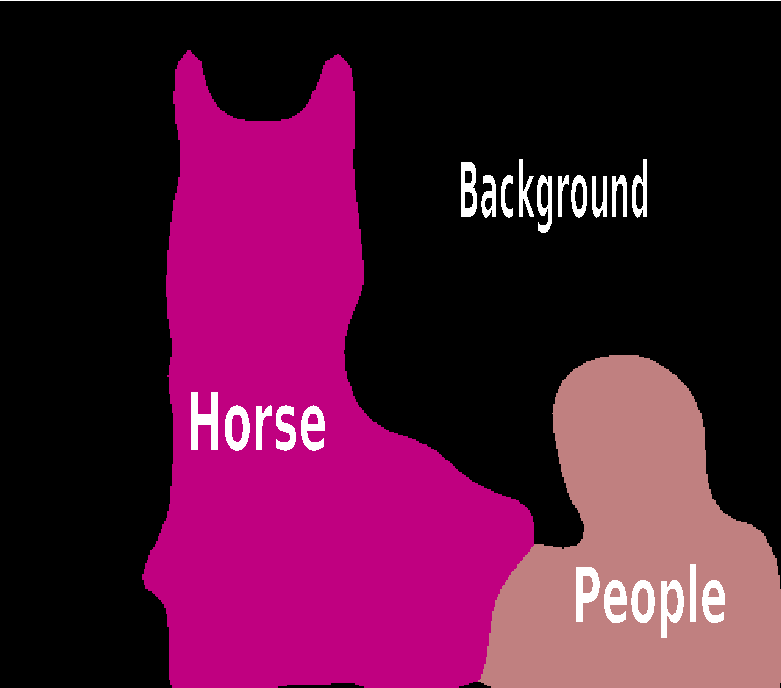
\includegraphics[width=.2\textwidth,height=.15\textwidth]{demo_images/example/2007_000799.pdf}
	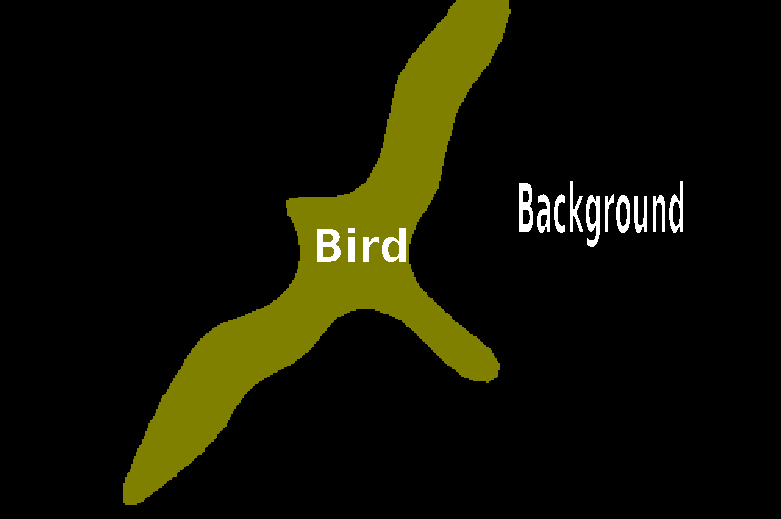
\includegraphics[width=.2\textwidth,height=.15\textwidth]{demo_images/example/2007_002094.pdf}
	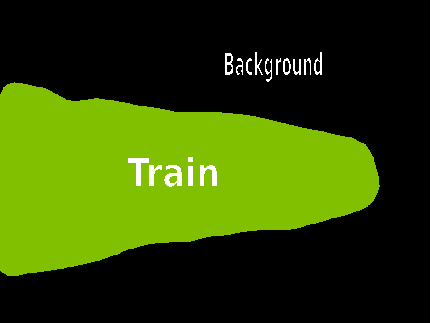
\includegraphics[width=.2\textwidth,height=.15\textwidth]{demo_images/example/2007_004483.pdf}
	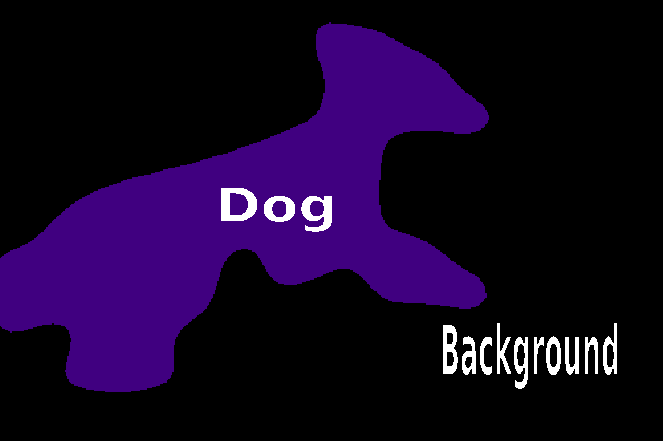
\includegraphics[width=.2\textwidth,height=.15\textwidth]{demo_images/example/2007_003194.pdf}
	\caption[语义图像分割的例子]{本文模型在VOC 2012验证集上的语义图像分割例子}
	\label{fig:example1}
\end{figure}